% ! TeX root = ./document.tex
\documentclass[9pt, aspectratio=169, handout]{beamer}
% ! TeX root = ../document.tex
\usepackage[utf8]{inputenc}
\usepackage{multicol}
\usepackage{pgfpages}
\usepackage{roboto}
\usepackage{PlayfairDisplay}
\usepackage{fontawesome5}
\usepackage[T1]{fontenc}
\usepackage[final]{pdfcomment}
\usepackage{minted}
\usepackage[backend=bibtex,style=alphabetic,sorting=none,doi=true,url=false]{biblatex} 
\usepackage{xargs}
% ! TeX root = ../document.tex
\usetheme{material}
\useDarkTheme
\usePrimaryRed
\useAccentGreen

% ! TeX root = ../document.tex

\title{
  {\fontfamily{\playfairfamily}\fontseries{black}\selectfont
    Towards Reinforcement Learning-based \\ Aggregate Computing
  }
}
\author[G.Aguzzi]{
  \textbf{Gianluca Aguzzi}\inst{1}, Roberto Casadei \inst{1}, Mirko Viroli \inst{1}
}
\institute{
  \inst{1}
  \texttt{Alma Mater Studiorum} -- Università di Bologna, Cesena, Italy
}
\talk{
  Talk @ COORDINATION 2022
}

\bibliography{biblio.bib}
\begin{document}
\begin{frame}[plain]
  \begin{backgroundblock} 
    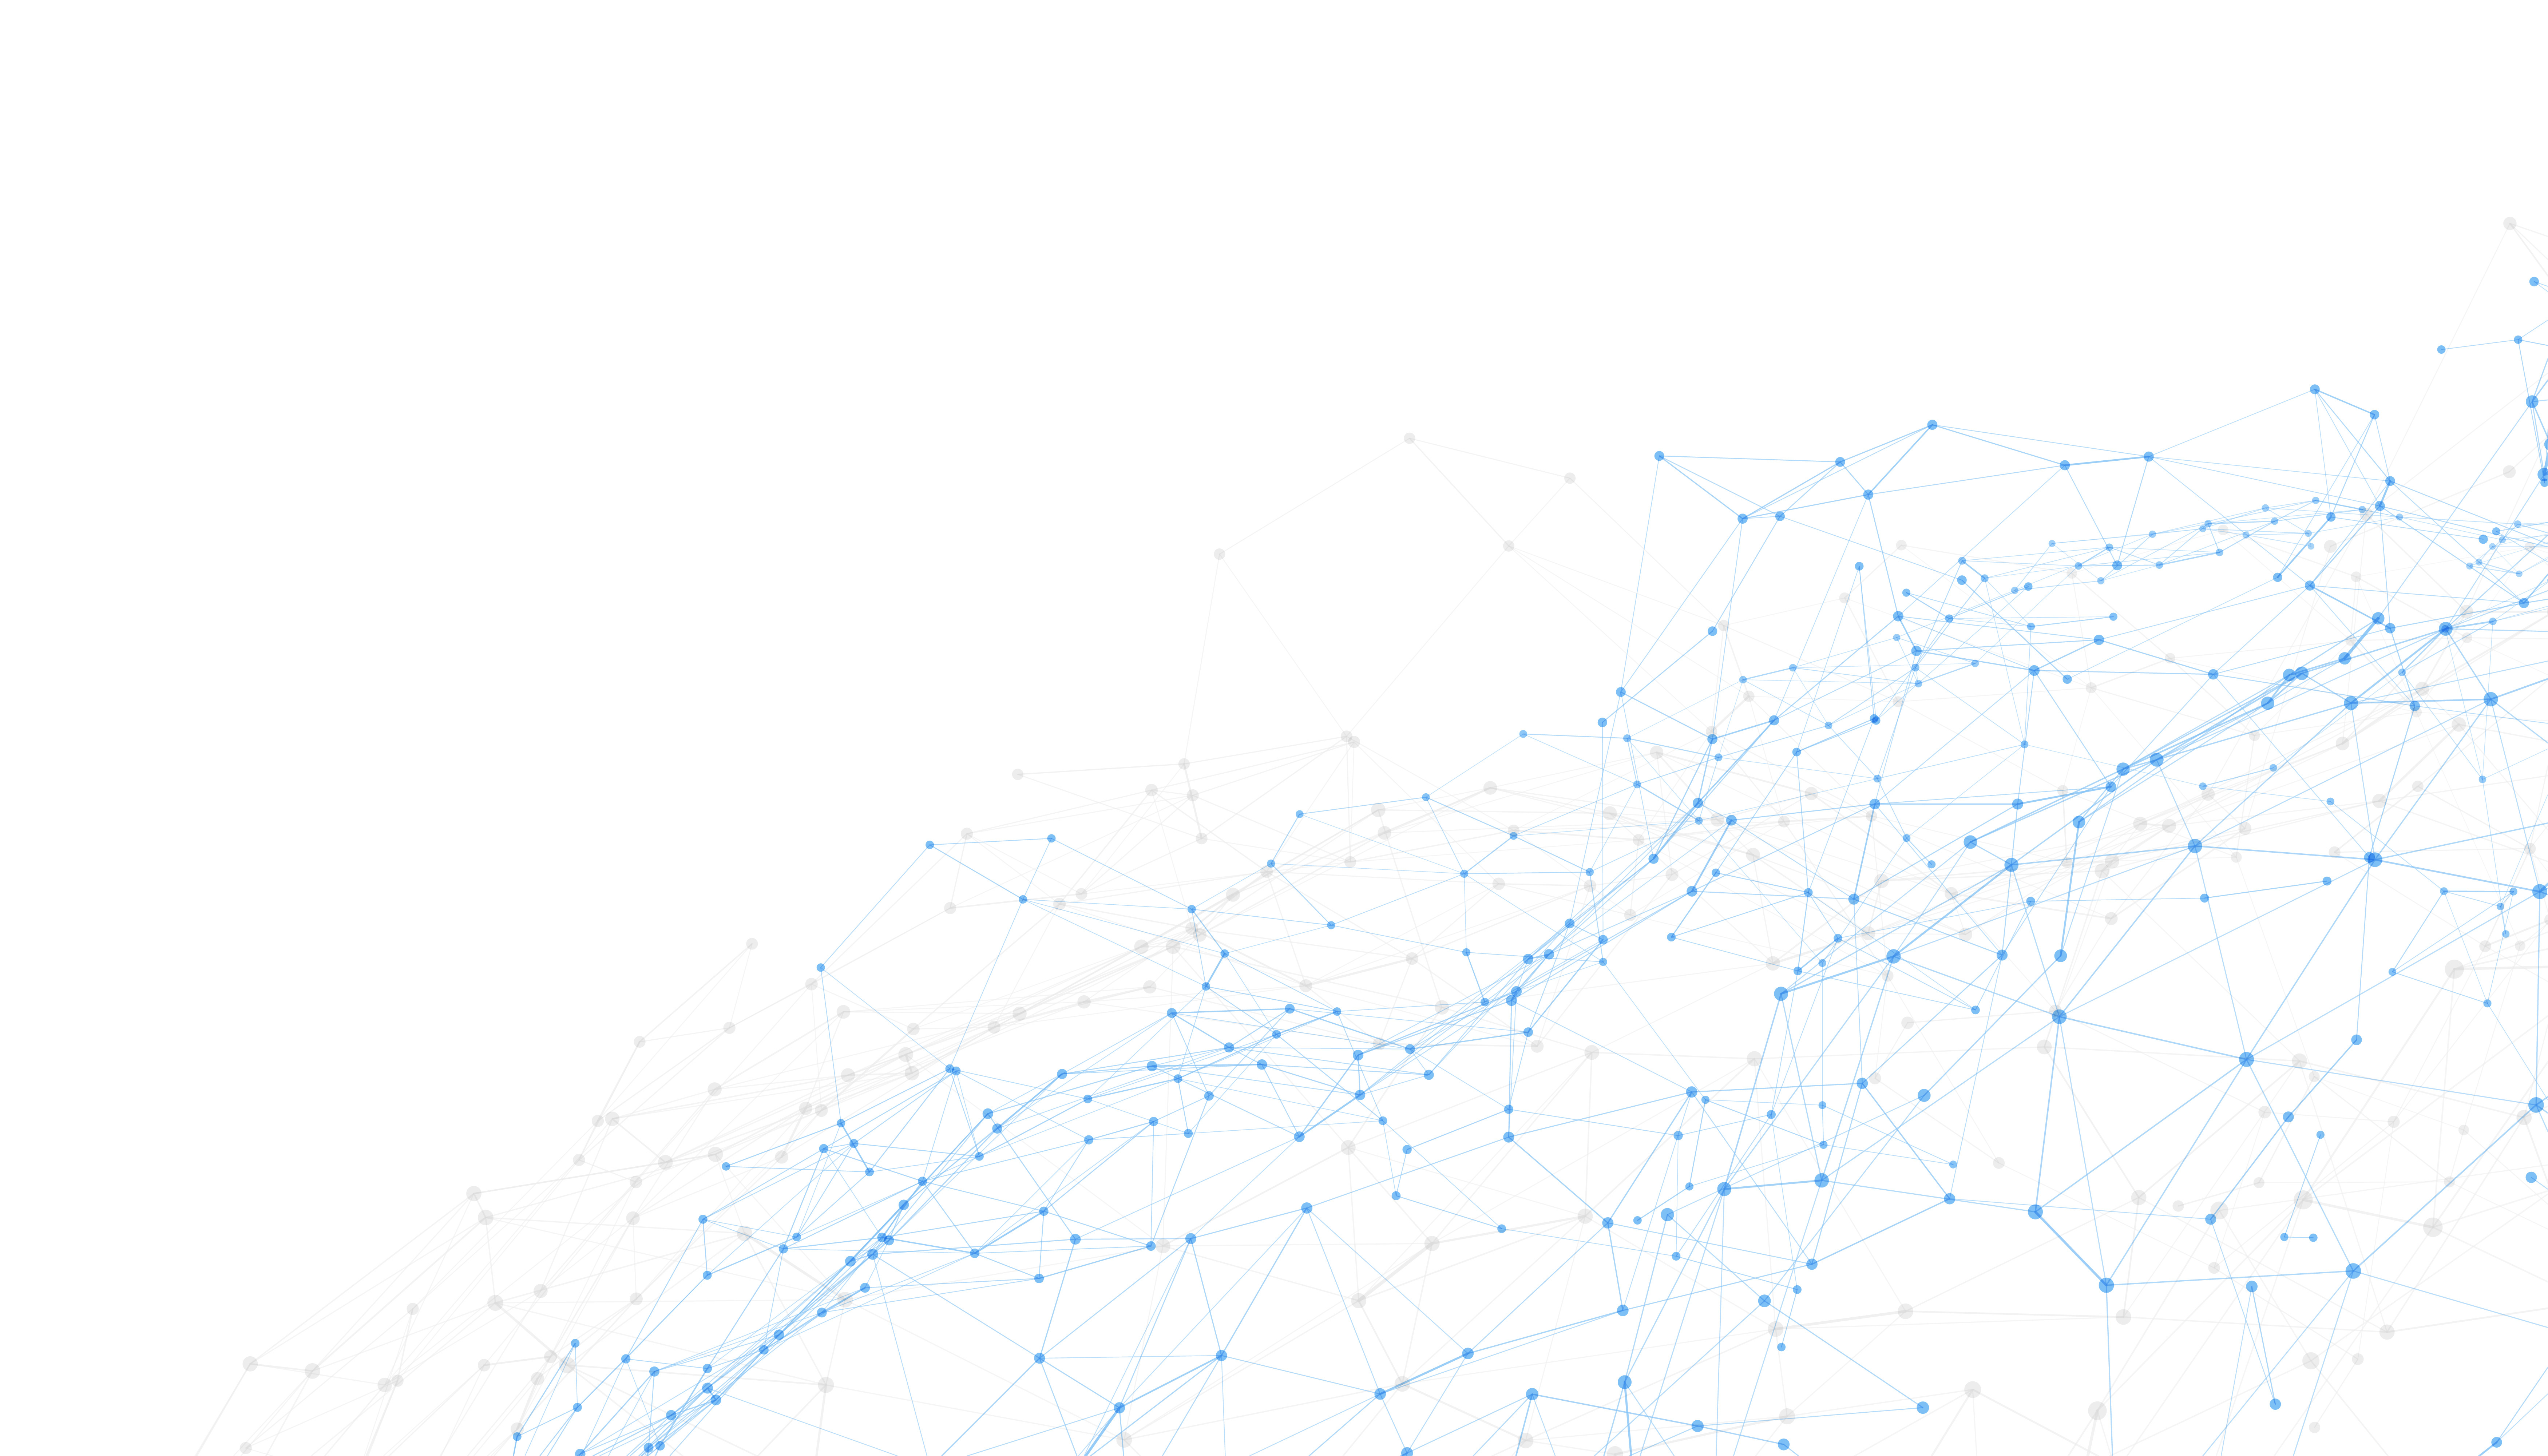
\includegraphics[width=\paperwidth]{img/network.jpg} 
  \end{backgroundblock} 
\titlepage
\end{frame}
\addtocounter{framenumber}{-1}
\section{Background}
\begin{frame}{Background}
  \begin{card}[Computing Systems of \textbf{Tomorrow} (Today?)]
    \begin{itemize}
      \item \highlight{Smart} things ``everywhere'' (\emph{pervasive}, \emph{ubiquitous}, \emph{collective} computing)
      \item Dense, layered and complex large-scale IT networks (\emph{cloud-fog-edge} computing)
      \item \highlight{Opportunistic} and \highlight{situated}-aware computing
    \end{itemize}
  \end{card}
  \begin{alarm}[Challenges]
    \begin{itemize}
      \item \highlight{Collective} \& \highlight{self-adaptive} behaviours \emph{\faArrowRight} Collective Adaptive Systems (CASs)
      \begin{itemize}
        \item \highlight{coordination}: how do entities interact to reach collective goals?
        \item \highlight{self-organization}: how to maintain a system in order?
      \end{itemize}
      \item Distributed control, local-to-global problem, openness, \dots
      \item \emph{How} can we program such kinds of systems?
    \end{itemize}
  \end{alarm}
\end{frame}

\begin{frame}{Aggregate Computing}
  \begin{cardTiny}
    \begin{itemize}
      \item <1-> A top-down global-to-local macro-programming approach to express \highlight{collective} \& \highlight{self-organising} behaviour~\cite{DBLP:conf/saso/BealVPD16}
      \item <2-> \highlight{Computational field} as a first-class abstraction for expressing system dynamics
      \begin{itemize}
        \item is a macro-abstraction that maps a set of devices over time to computational values
        \item [\success{\faThumbsUp}] \highlight{Functional approach}: distributed program expressed as a functional application through computational fields
      \end{itemize}
    \end{itemize}
  \end{cardTiny}
  \begin{multicols}{2}
    \begin{card}[Benefits]
      \begin{itemize}
        \item Programs expressed thinking about macro-properties
        \item \highlight{Scale-independent} \& \highlight{self-stabilising} collective behaviours
      \end{itemize}
    \end{card}
    \begin{cardTiny}
      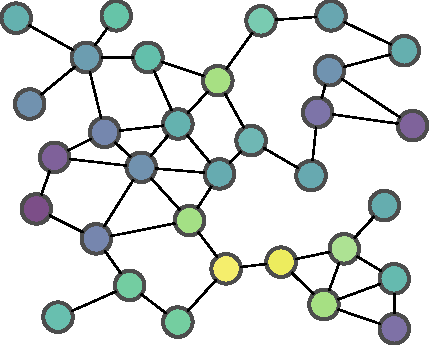
\includegraphics[width=0.45\textwidth]{img/discrete.pdf}
      \hfill
      %\parbox[c]{0.1\textwidth}{\Large  \vspace*{\fill} \strut \faArrowRight \vspace*{\fill}}
      \parbox[c]{1em}{\color{primary}\vspace*{-6em}\Large \faArrowRight}
      \hfill
      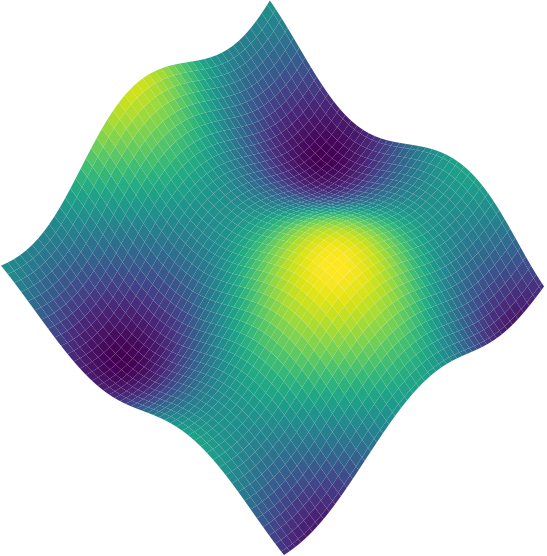
\includegraphics[width=0.38\textwidth]{img/viridis-result.png}
    \end{cardTiny}
  \end{multicols}
\end{frame}
\begin{frame}[fragile]{Aggregate Computing -- In a nutshell}
  \begin{multicols}{2}
    \begin{card}[Gradient]
    \begin{minted}{scala}
val gradient = rep(Inf)(distance =>
mux(source){0.0}/*else*/{
  includingSelf.
    minHood(nbr{distance} + nbrRange)
})
    \end{minted}
    \centering
    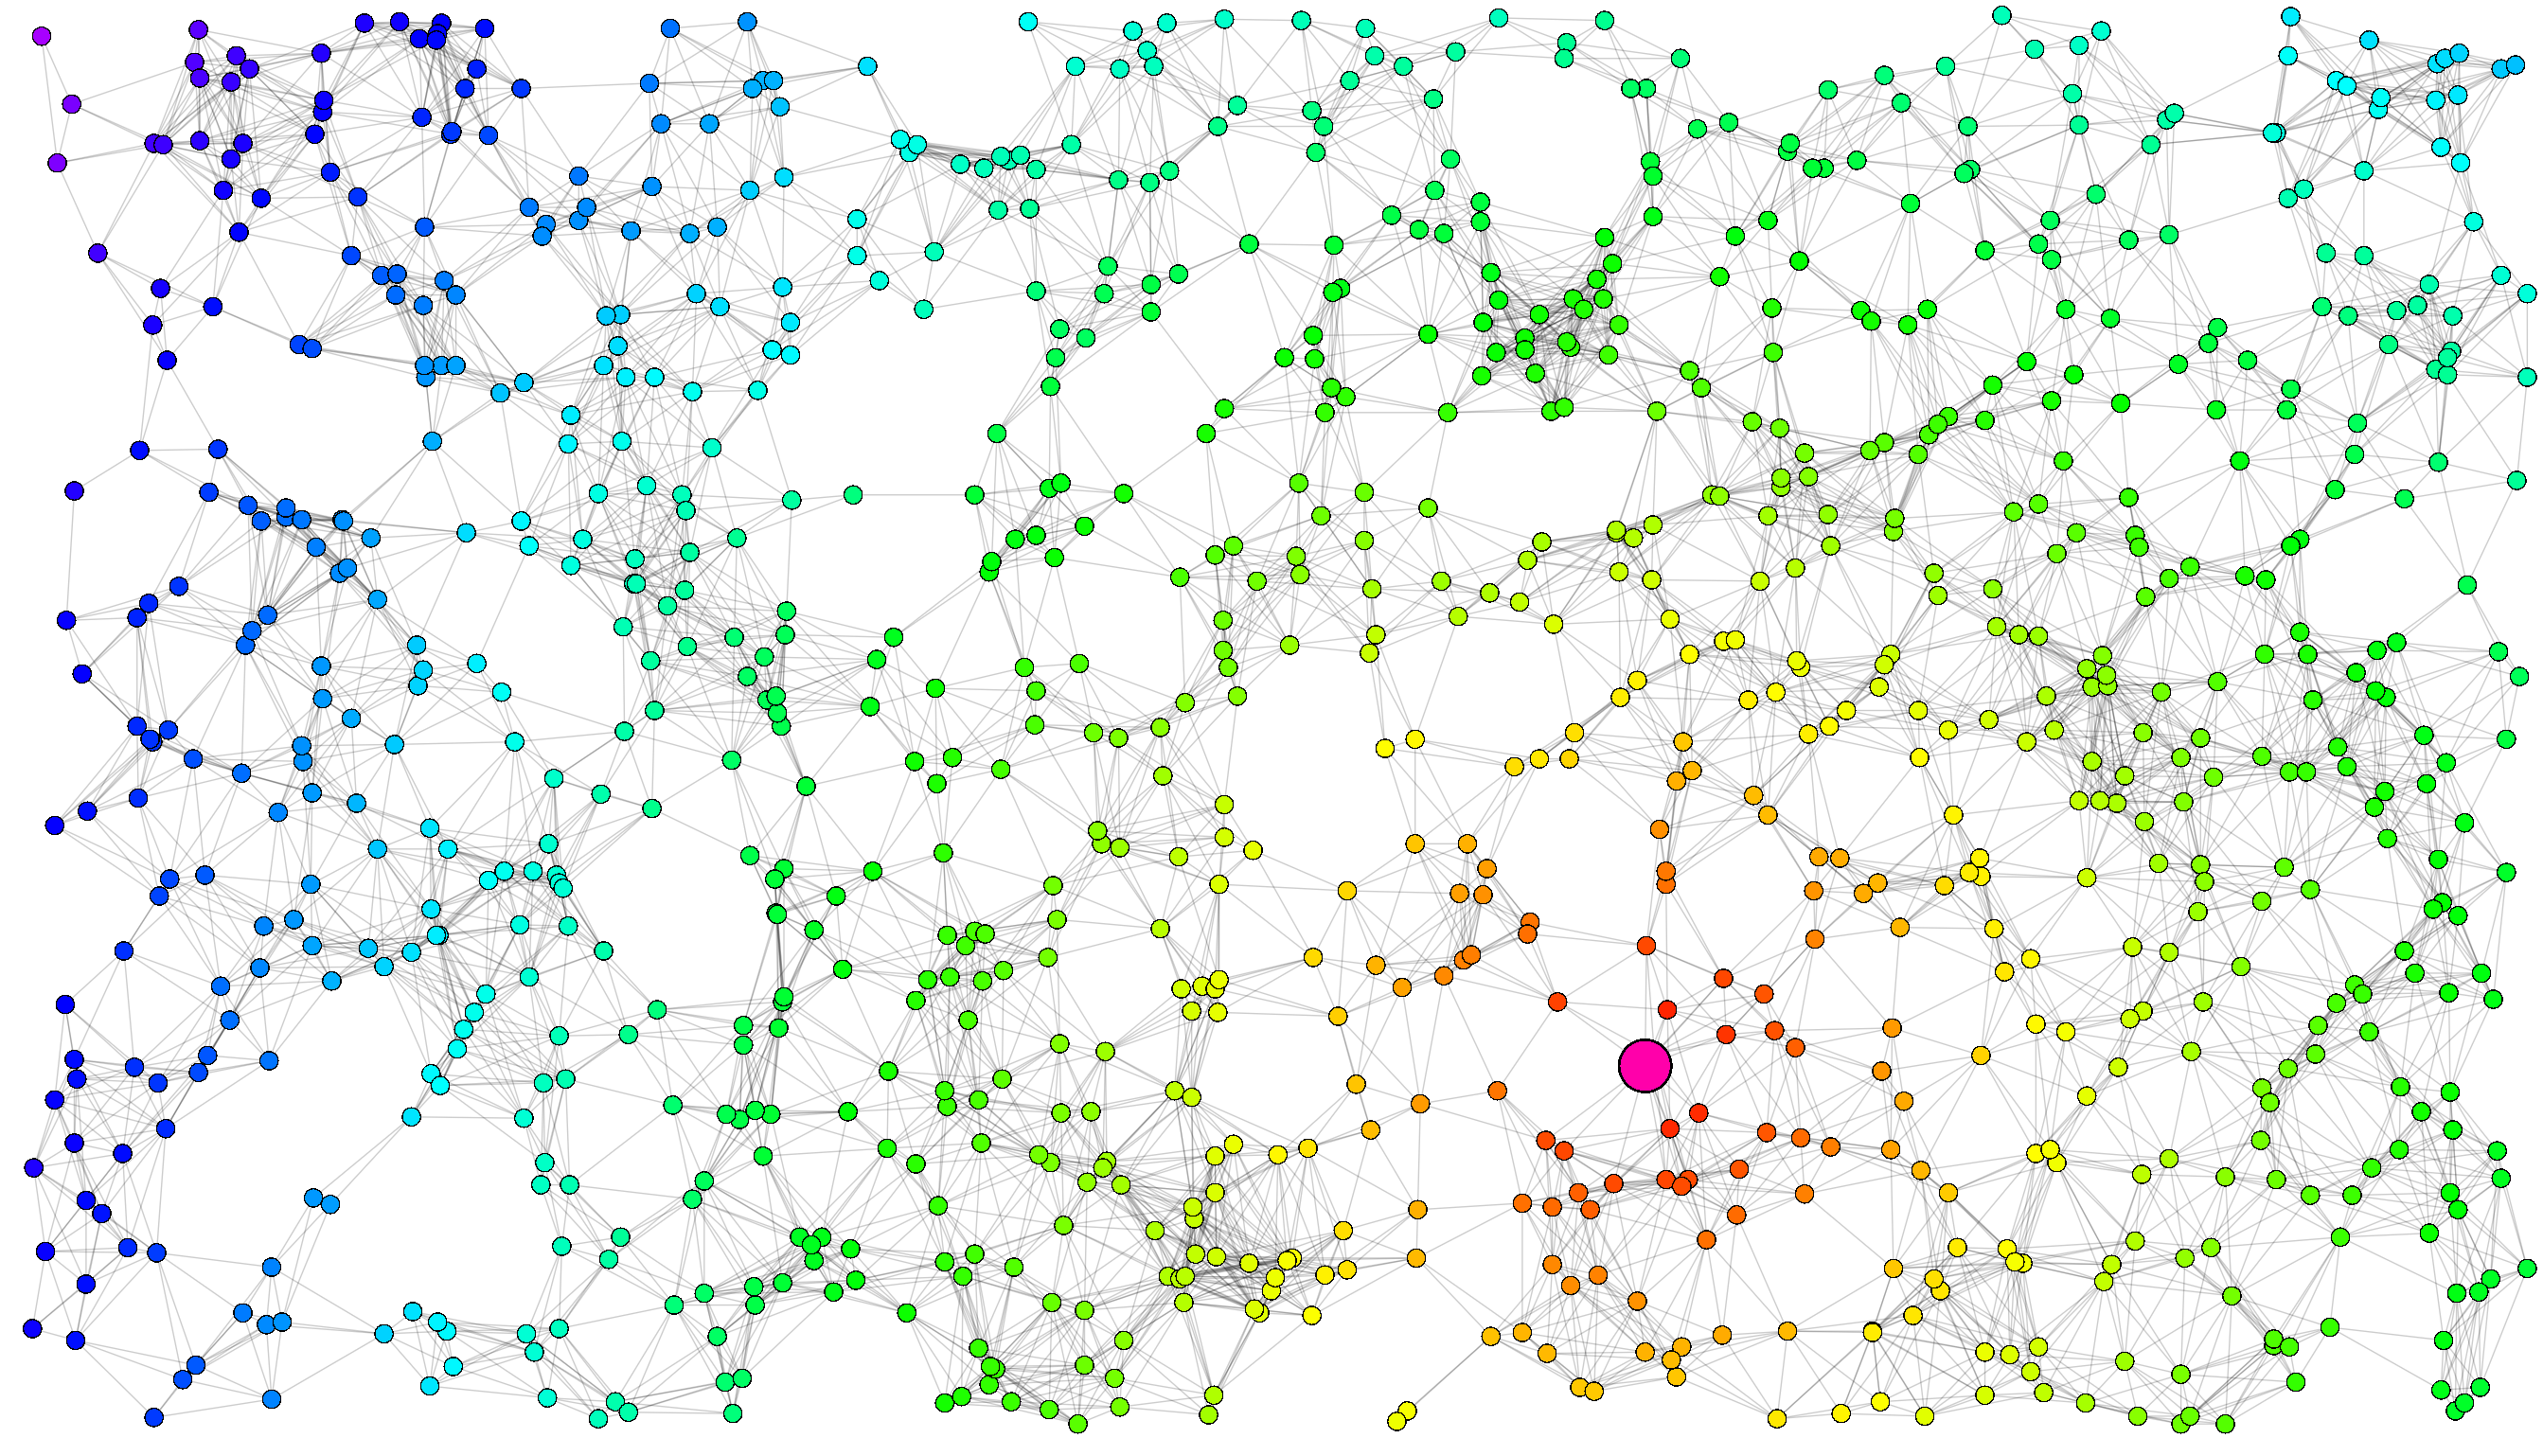
\includegraphics[width=0.7\linewidth]{img/result-gradient.png}
    \end{card}
    \begin{card}[Distributed sensing]
    \begin{minted}{scala}
val leader = S(radius)
val potential = distanceTo(leader)
val mean =
  collectMean(potential, temperature)
broadcast(leader, mean)
  \end{minted}  
  \centering
  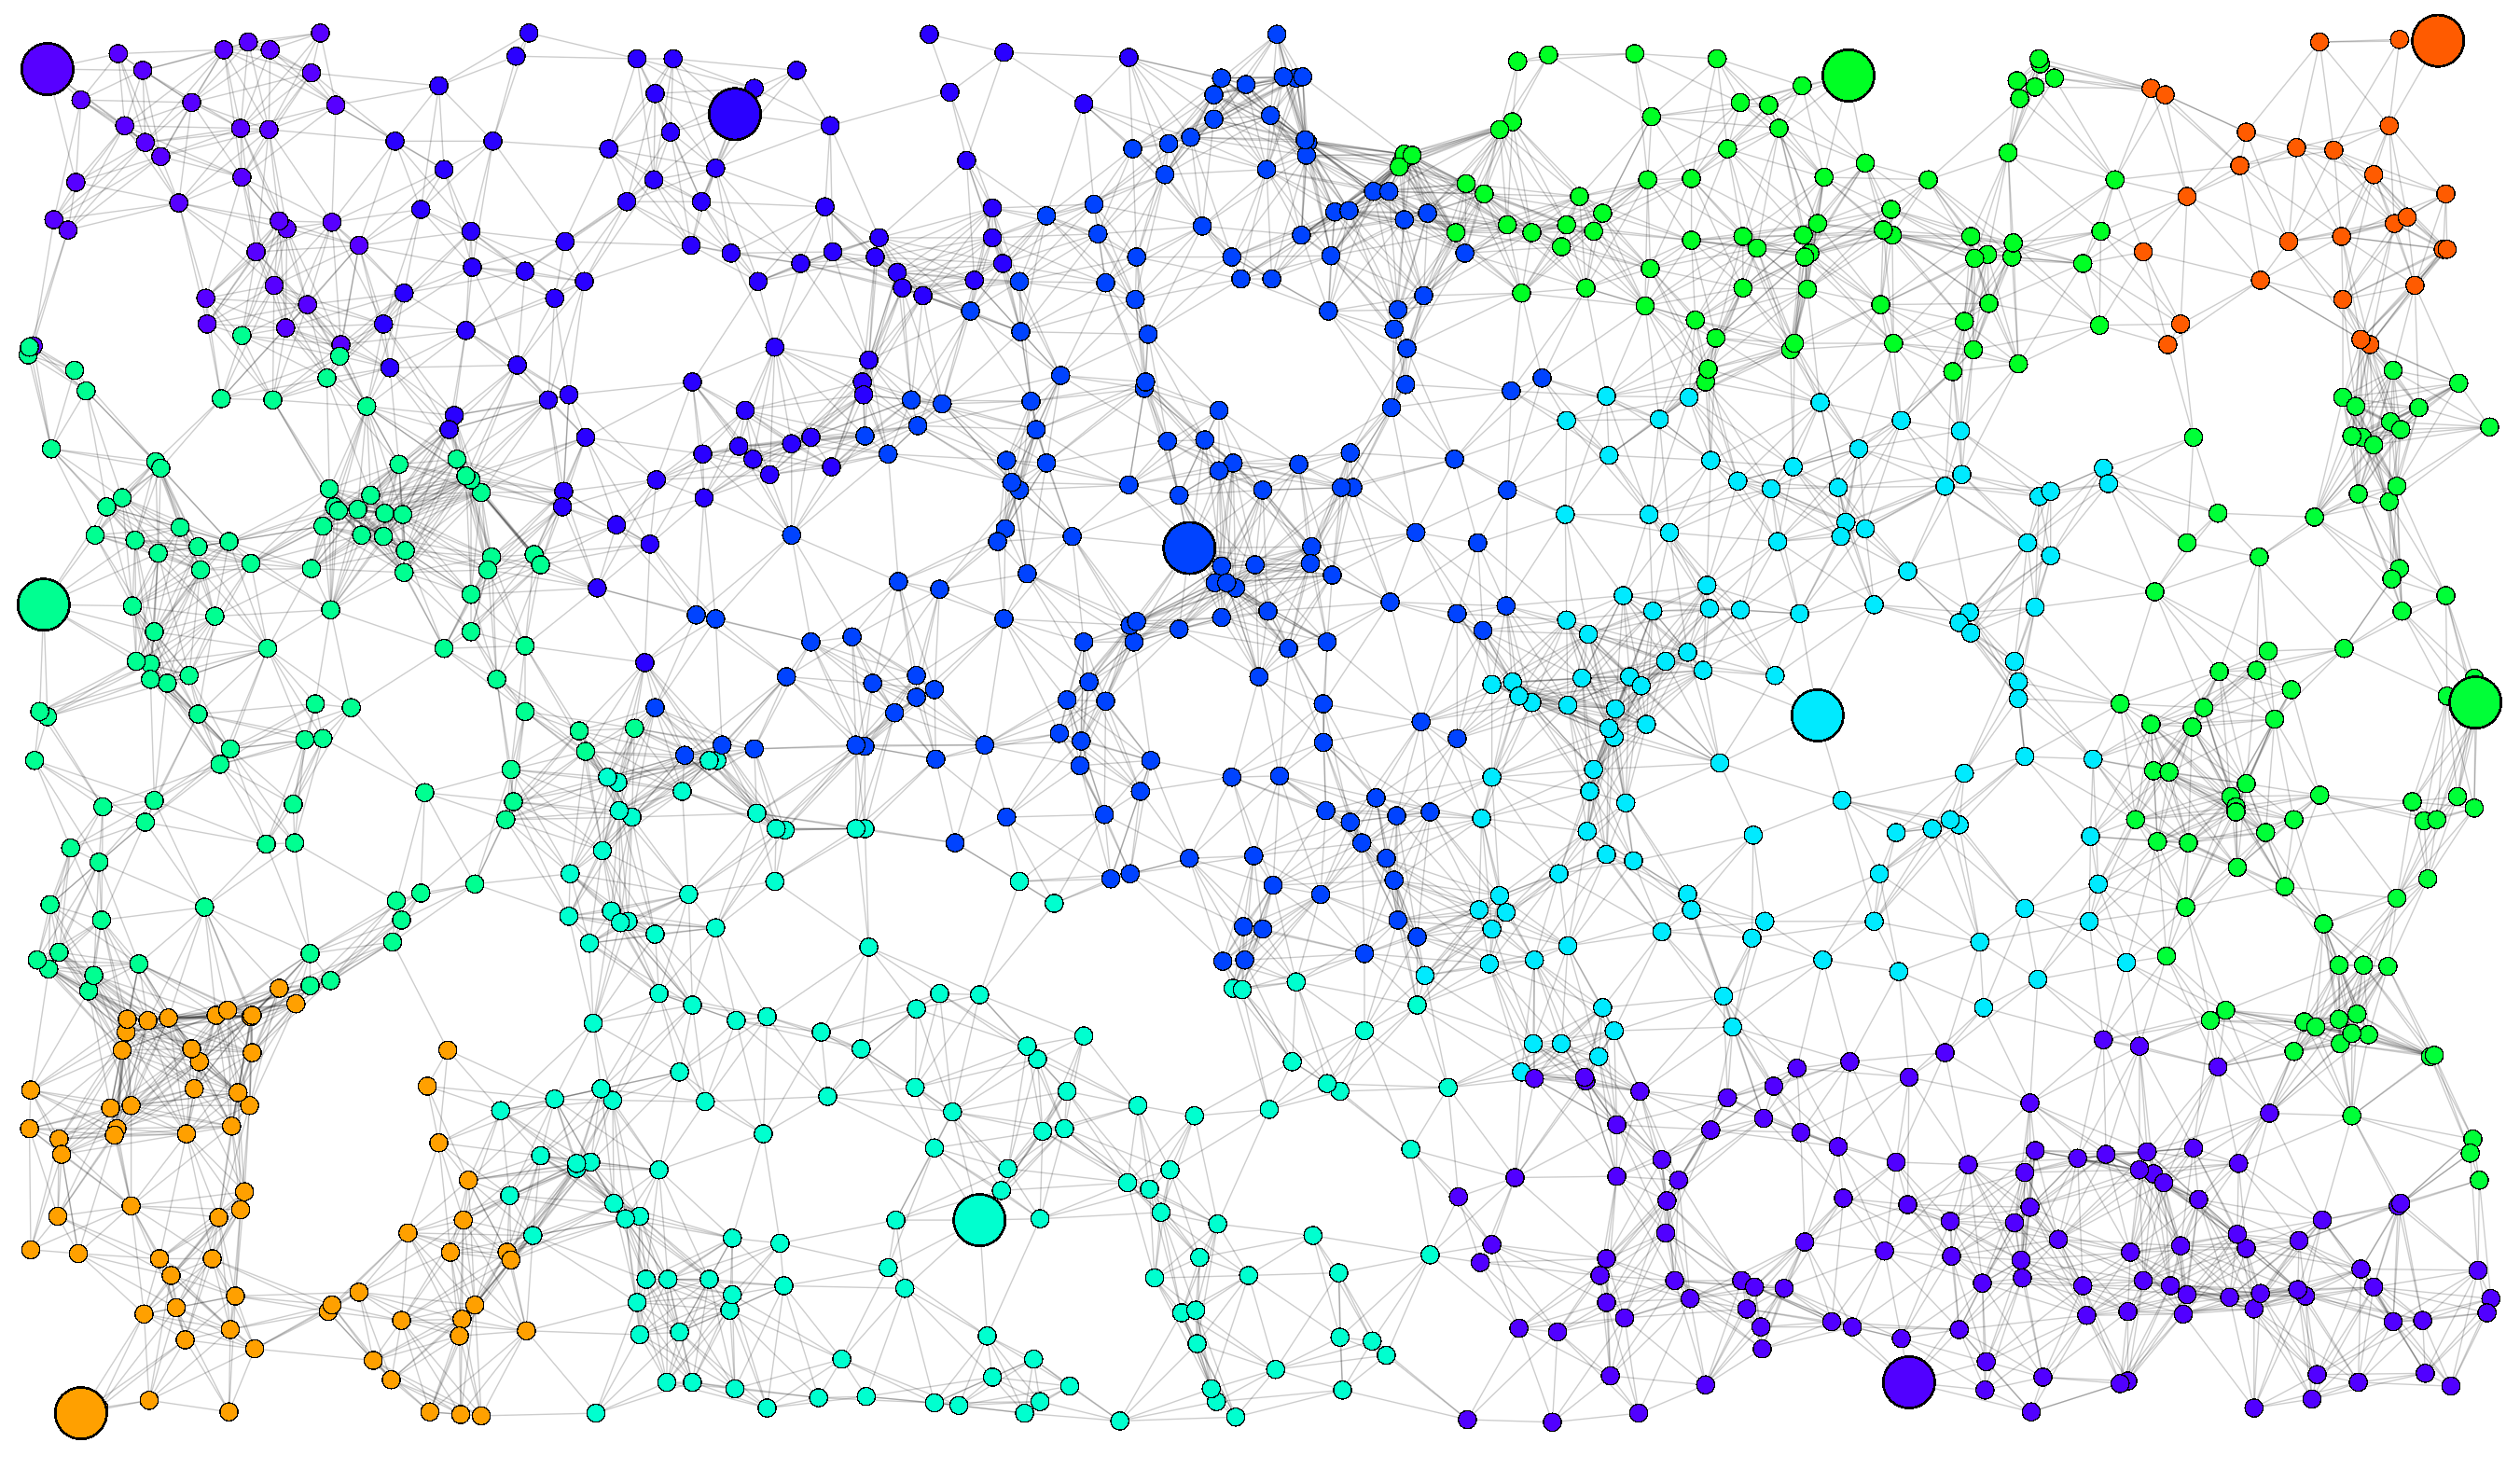
\includegraphics[width=0.68\linewidth]{img/distributed-sensing.png}   
  \end{card}
  \end{multicols}
\end{frame}
\begin{frame}{Aggregate Computing -- Execution model}
  \begin{columns}
    \begin{column}{0.49\textwidth}
      \begin{card}[Round Execution]
        \begin{enumerate}
          \item \highlight{context acquisition}
          \begin{itemize}
            \item sensors data
            \item messages from neighbours
            \item local state
          \end{itemize}
          \item \highlight{program evaluation} is a function from context to \emph{export}
          \item \highlight{export sharing} to the neighbours
          \item \highlight{actuations} using export
        \end{enumerate}
      \end{card}
    \end{column}
    \begin{column}{0.51\textwidth}  
      \begin{cardTiny}
        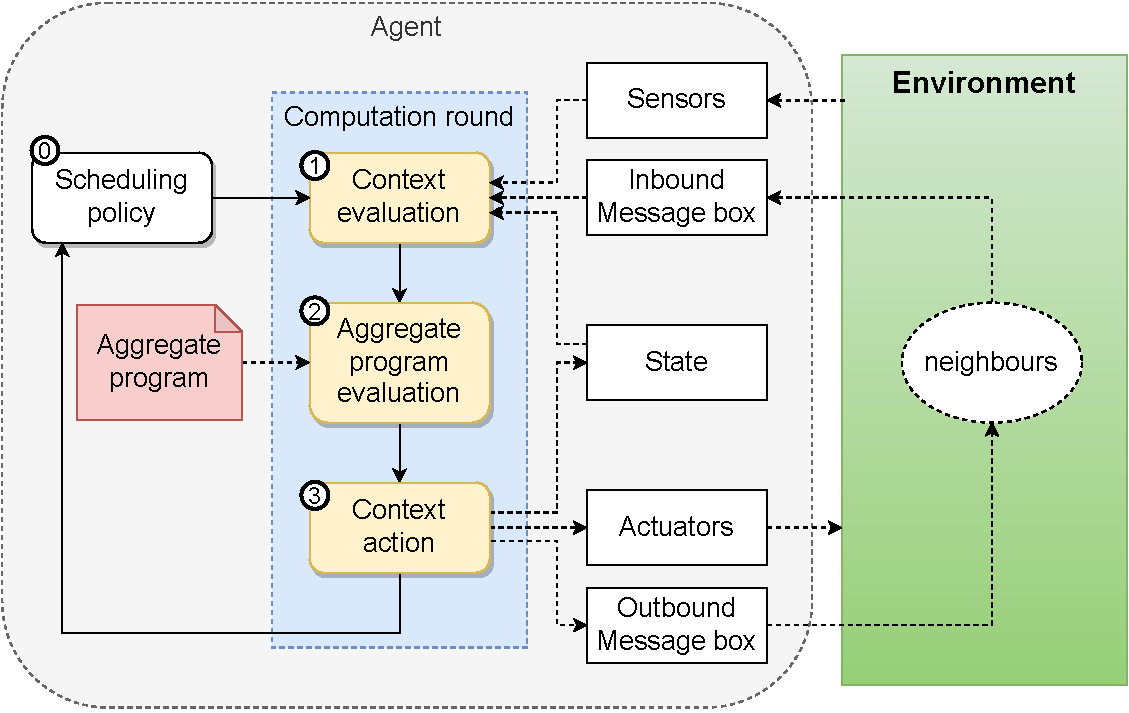
\includegraphics[width=\textwidth]{img/aggregate-agent-control-architecture.drawio.pdf}    
      \end{cardTiny}
    \end{column}
  \end{columns}
\end{frame}
\begin{frame}{Aggregate Computing -- State of the art}
\begin{card}[Research trends]
  \begin{itemize}
    \item \highlight{Coordination algorithms}: \emph{gradients}, leader election (\highlight{S}), distributed sensing, \dots
    \item \textbf{Execution platform \& non-functional aspects}: Aggregate program deployment (pulverised architecture), collective program scheduling (distributed schedulers) and trust.
  \end{itemize}
\end{card}
\begin{alarm}[Challenges]
  \begin{itemize}
    \item The self-healing gradient case
    \begin{itemize}
      \item this algorithm could suffer from several issues~\cite{DBLP:conf/saso/AudritoCDV17}
      \begin{itemize}
        \item[\faArrowRight] non-smooth output
        \item[\faArrowRight] slow-rising value
        \item[\faArrowRight] speed bias
      \end{itemize}
      \item several heuristics \& algorithms (CRF, Flex, BIS, \dots) have been proposed \dots
      \item \dots but can we \emph{learn} how to handle these situations?
    \end{itemize}
  \end{itemize}
\end{alarm}
\end{frame}
\section{Proposed approach}
\begin{frame}{Reinforcement Learning-based Aggregate Computing}
\begin{cardTiny}
  \begin{itemize}
    \item \highlight{Idea}: maintaining the high-level interface of Aggregate computing
    \begin{itemize}
      \item[\faArrowRight] strong foundational discovery (\emph{self-stabilisation} \& \emph{eventual consistency})
      \item[\faArrowRight] control on application description \& logic
      \item[\faArrowRight] the programming model ensures \emph{composability}
    \end{itemize}
    \item  while use \emph{Reinforcement Learning} for:
    \begin{itemize}
      \item[\faArrowRight] increasing adaptivness of collective behaviour
      \item[\faArrowRight] \emph{learning} effective collective strategy \emph{by doing}
    \end{itemize}
  \end{itemize}
\end{cardTiny}

\begin{card}[Integration perspective]
  \begin{itemize}
    \item \emph{Coordination algorithms}: learning used to fill \highlight{holes} in a template program with actions determined through search (kind of sketching~\cite{solar2008program-synthesis-sketching})
    \item Execution framework: learning used as a mechanism to improve non-functional aspects (e.g., computational efficiency, \dots)
  \end{itemize}
\end{card}
\end{frame}
\begin{frame}{Execution Model -- Revised}
  \begin{columns}
    \begin{column}{0.49\textwidth}
      \begin{card}[Round Execution]
        \begin{itemize}
          \item The loop ``acquisition -- evaluation -- sharing -- actuation'' remains
          \item The state and the reward
          \begin{itemize}
            \item created from the context (environment)
          \end{itemize}
          \item The \emph{policy}
          \begin{itemize}
            \item is evaluated along the aggregate program
            \item produces an action piggybacked on the export
          \end{itemize}
        \end{itemize}
      \end{card}
    \end{column}
    \begin{column}{0.57\textwidth}  
      \begin{cardTiny}
        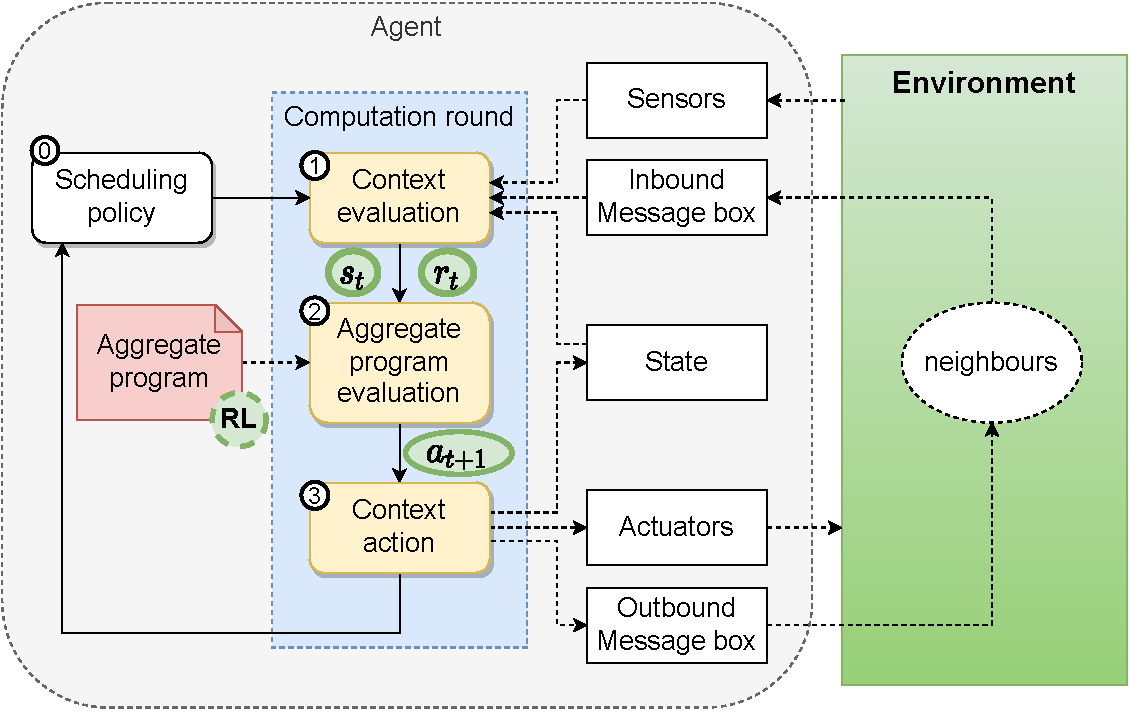
\includegraphics[width=\textwidth]{img/aggregate-agent-control-architecture-rl.pdf}    
      \end{cardTiny}
    \end{column}
  \end{columns}
\end{frame}
\begin{frame}{Learning Settings}
  \begin{cardTiny}
    \begin{itemize}
      \item \highlight{Multi-agent system}: each agent interferes with the system-wide learning process (\emph{non-stationary environment})
      \item \highlight{Homogenous behaviour}~\cite{DBLP:journals/aamas/PanaitL05}: In the context of Aggregate Computing we could consider homogenous behaviour
      \begin{itemize}
        \item nodes should run the same aggregate program
        \item then we could search \highlight{one} policy for the entire aggregate
      \end{itemize}
      \item \highlight{Centralised Traning Decentralised Execution}~\cite{DBLP:phd/ethos/Foerster18}
      \begin{itemize}
        \item learning done by means of simulations (\emph{global view})
        \item the policy is shared then throughout the whole system
        \item[\faThumbsUp] global information at training time that influences distributed policy at runtime
      \end{itemize}
    \end{itemize}
  \end{cardTiny}
  \centering
  \cardImg{img/algorithm-learning.pdf}{0.65\textwidth}
\end{frame}
\section{Case study}
\begin{frame}[allowframebreaks, fragile]{Evaluation: the slow-rising problem}
  \begin{card}[Problem Description]
    \begin{itemize}
      \item The self-healing gradient output is built via a repeated minimisation of neighbours' contributions
      \item[\success{\faThumbsUp}] the system handles well the situations when the output needs to drop
      \begin{itemize}
        \item a new source enters the system
      \end{itemize}
      \item[\failure{\faThumbsDown}] the system reacts slowly when the output needs to rise
      \begin{itemize}
        \item a source node turns off
      \end{itemize}
    \end{itemize}
  \end{card}
  \begin{columns}
    \begin{column}{0.26\textwidth}
      \cardImg{img/slow-rising-problem.pdf}{\textwidth}
    \end{column}
    \begin{column}{0.26\textwidth}
      \cardImg{img/slow-rising-problem-1.pdf}{\textwidth}
    \end{column}
    \begin{column}{0.26\textwidth}
      \cardImg{img/slow-rising-problem-2.pdf}{\textwidth}
    \end{column}
  \end{columns}
  \begin{card}[Solution Design]
    \begin{itemize}
      \item Inspired from Constraint and Restoring Force~\cite{DBLP:conf/sac/BealBVT08} (CRF)
      \item Based on Q-Learning~\cite{DBLP:journals/ml/WatkinsD92} (particularly on Hysteretic Q-Learning~\cite{DBLP:conf/iros/MatignonLF07})
      \item \emph{Idea}: learn when the output should increase even if the neighbours bound the result
      \item Program template: \mintinline{scala}{rep(infinity) { g => mux(source) { 0 } { ??? /*hole*/ } }}
      \item Reinforcement Learning problem definition:
      \begin{itemize}
        \item \emph{State}: a window of minimum and maximum delta of neighbours output
        \begin{itemize}
          \item[\faArrowRight] Track the output evolution
        \end{itemize}
        \item \emph{Actions}: define when the output should increase
        \begin{itemize}
          \item[\faArrowRight] \texttt{ConsiderNeighborhood}: use the standard gradient evaluation
          \item[\faArrowRight] \texttt{Ignore(velocity)}: increase the output following the velocity described
        \end{itemize}
        \item \emph{Reward}: 0 if the output is the same of an oracle, -1 otherwise
        \begin{itemize}
          \item[\faArrowRight] push agents to reach a condition when the output is similar to oracle predictions
        \end{itemize}
      \end{itemize}
    \end{itemize}
  \end{card}
\framebreak
  \begin{card}[Simulation Setup]
    \begin{itemize}
      \item 1000 episodes are used to train the policy ($\epsilon-greedy$ policy), 200 episodes to evaluate the performance (i.e., greedy policy)
      \item The policy is considered in two environments 
      \begin{itemize}
        \item one with 200 agents arranged in a grid
        \item another with 40 agents in a similar grid
        \item we would check the effect of node size in our solution
      \end{itemize}
      \item Solution error evaluated as the mean difference from the output produced with Reinforcement Learning and with the oracle
    \end{itemize}
  \end{card}  
  \begin{columns}
    \begin{column}{0.3\textwidth}
      \cardImg{img/result-rectangle.png}{\textwidth}
    \end{column}
    \begin{column}{0.38\textwidth}
      \cardImg{img/result-rectangle-low.png}{\textwidth}
    \end{column}  
  \end{columns}
  \begin{card}[Results]
    \begin{itemize}
      \item The system eventually learns a policy that has a performance comparable to CRF
      \item The policy is independent of the nodes that partecipates in the system
      \item Result are reproducible following the instruction on the code repository\footnote[frame]{\url{https://github.com/cric96/experiment-2022-acsos-round-rl}}
      \begin{itemize}
        \item The simulations are performed using Alchemist~\cite{alchemist-jos2013} and ScaFi~\cite{DBLP:conf/isola/CasadeiVAD20} 
      \end{itemize}
    \end{itemize}
  \end{card}
  \begin{multicols}{3}
    \cardImg{img/mean-error-left.pdf}{0.29\textwidth}
    \cardImg{img/output-few-nodes.pdf}{0.29\textwidth}
    \cardImg{img/output-many-nodes.pdf}{0.29\textwidth}
  \end{multicols}
\end{frame}
\section{Conclusion}
\begin{frame}{Conclusion}
  \begin{cardTiny}
  \begin{itemize}
    \item We successfully integrate a programming approach for Collective Adaptive Systems with and Reinforcement Learning
    \begin{itemize}
      \item \emph{goal}:  fostering the design of collective adaptive behaviour
    \end{itemize}
    \item Paper focus: Reinforcement Learning for improving Aggregate Computing building blocks
    \begin{itemize}
      \item The approach is evaluated through a case study: the slow-rising of self-healing gradient 
    \end{itemize}
  \end{itemize}
  \end{cardTiny}
  \begin{card}[Future works]
    \begin{itemize}
      \item Applying learning to other building blocks (leader election, distributed sensing, \dots)
      \item Move to continuous state/action spaces
      \item Use Machine Learning at the execution platform too for
      \begin{itemize}
        \item reducing the power consumption
        \item supporting opportunistic reconfiguration
        \item reducing the data amount exchanged between nodes
      \end{itemize}
    \end{itemize}
  \end{card}
\end{frame}

\begin{frame}[allowframebreaks]
  \frametitle{References}
  \printbibliography
\end{frame}
\end{document}
